\documentclass[solution,addpoints,12pt]{exam}
\usepackage{amsmath}
\usepackage{amsthm}
\usepackage{amssymb}
\usepackage{tikz}
\usepackage{animate}
\usepackage{hyperref}
\usepackage{booktabs}
\newtheorem{theorem}{Theorem}
\newtheorem{lemma}[theorem]{Lemma}
\usepackage{mathtools}
\DeclarePairedDelimiter\ceil{\lceil}{\rceil}

\newenvironment{Solution}{\begin{EnvFullwidth}\begin{solution}}{\end{solution}\end{EnvFullwidth}}

\printanswers
%\unframedsolutions
\pagestyle{headandfoot}

%%%%%%%%%%%%%%%%%%%%%%%%%%%%%%%%%%%%%%%%%%%%%%%%%%%%%%
%%%%%%%%%%%%%%%%%%% INSTRUCTIONS %%%%%%%%%%%%%%%%%%%%%
% * Fill in your name and roll number below

% * Answer in place (after each question)

% * Use \begin{solution} and \end{solution} to typeset
%   your answers.
%%%%%%%%%%%%%%%%%%%%%%%%%%%%%%%%%%%%%%%%%%%%%%%%%%%%%%
%%%%%%%%%%%%%%%%%%%%%%%%%%%%%%%%%%%%%%%%%%%%%%%%%%%%%%

% Fill in the details below
\def\studentName{\textbf{Name:Avani Shukla\hspace{0mm}}}
\def\studentRoll{\textbf{Roll No:CS18M052\hspace{0mm}}}

\firstpageheader{CS 7015 - Deep Learning - Assignment 1}{}{\studentName, \studentRoll}
\firstpageheadrule

\newcommand{\brac}[1]{\left[ #1 \right]}
\newcommand{\curly}[1]{\left\{ #1 \right\}}
\newcommand{\paren}[1]{\left( #1 \right)}
\newcommand{\card}[1]{\left\lvert #1 \right\rvert}

\allowdisplaybreaks
\begin{document}
\textbf{Instructions:}
\begin{itemize}
    \itemsep0em
    \item This assignment is meant to help you grok certain concepts we will use in the course. Please don't copy solutions from any sources.
    \item Avoid verbosity.
    \item The assignment needs to be written in latex using the attached tex file. The solution for each question should be written in the solution block in space already provided in the tex file. \textbf{Handwritten assignments will not be accepted.}
    
\end{itemize}

\begin{questions}

\question \textbf{Partial Derivatives}
          \newline
          \begin{parts}
   

        \part Find the derivative of $g(\rho)$ with respect to $\rho$ where $g(\rho)$ is given by,
      \[ g(\rho) = \frac{1}{2} \rho log\frac{\rho}{\rho+\hat{\rho}} + \frac{1}{2} \hat{\rho} log\frac{\hat{\rho}}{\rho+\hat{\rho}} \]
      (You can consider $\hat{\rho}$ as constant)
      \begin{solution}
      \vspace*{0mm}
      The derivative of $g(\rho)$ with respect to $\rho$ can be found as follows:
      \begin{align*}
        {g}'(\rho) &=  \frac{d}{d\rho}( \frac{1}{2} (\rho log\rho - \rho log(\rho+\hat{\rho})) + \frac{1}{2} \hat{\rho} (log\hat{\rho} - log(\rho+\hat{\rho})))\\
       &=  \frac{1}{2} (\frac{d\rho}{d\rho} log\rho + \rho \frac{d}{d\rho}(log\rho) - \rho \frac{d}{d\rho}(log(\rho+\hat{\rho})) - \frac{d\rho}{d\rho} log(\rho+\hat{\rho})) - \frac{1}{2} \hat{\rho}  \frac{d}{d\rho} (log(\rho+\hat{\rho})) \\
       &  \hspace*{112mm}(By\,Product\,Rule)\\ 
       &= \frac{1}{2} (log\rho + \frac{\rho}{\rho} - \frac{\rho}{\rho+\hat{\rho}} - log(\rho+\hat{\rho}) - \frac{\hat{\rho}}{\rho+\hat{\rho}})\\
       &= \frac{1}{2} log(\frac{\rho}{\rho+\hat{\rho}})
      \end{align*}
     
      \end{solution}
            \part Consider the following computation ,
                  \begin{center}
                  \hspace*{-15mm}
                    \tikzstyle{neuron1}=[circle,draw=blue!50,fill=blue!20,thick,minimum size=1mm]
                    \tikzstyle{neuron2}=[circle,draw=blue!50,fill=blue!20,thick,minimum size=6mm]
                    \tikzstyle{input}=[circle,draw=black!50,fill=black!20,thick,minimum size=6mm]
                    \begin{tikzpicture}
                        \node [neuron1] (neuron1) at (0.1,6)  {$\frac{1 + tanh(wx+b)}{2}$} ;
                        \node [neuron2] (neuron2) at (4,6)  {$sigm(z)$} ;
                        \node (input1) at (-3,6)  {$x$};
                        \node (input0) at (-3,5)  {$1$};
                        \node (output0) at (6,6)  {$f(x)$};
                        \node (formula) at (0,4) {where $ z = \frac{1 + tanh(wx+b)}{2}$ and $f(x) = sigm(z)$};
                        \node (formula2) at (0,3) {by definition : $sigm(z) = \frac{1}{1+e^{-z}}$ and $tanh(z) = \frac{e^{z} - e^{-z}}{e^{z} + e^{-z}} $ };
                        \draw [->] (input0) -- (neuron1);
                        \draw [->] (input1) -- (neuron1);
                        \draw[->] (neuron1) -- (neuron2);
                        \draw [->] (neuron2) -- (output0);
                        \node (label) at (2.3,6.3) {$z$};
                    \end{tikzpicture}
                  \end{center}
                  The value $L$ is given by, 
                  \[ 
                     L = - y \log (f(x))          \]
                  Here, $x$ and $y$ are constants and $w$ and $b$ are parameters that can be modified.
                  In other words, $L$ is a function of $w$ and $b$.

                  Derive the partial derivatives, $\frac{\partial L}{\partial w}$ and $\frac{\partial L}{\partial b}$.
   
              \begin{solution}
                \vspace*{0mm}
                Given, $L = - y \log (f(x)) = - y \log (sigm(z))$ \\

                The partial derivative of $L$ w.r.t $w$ is given by $\frac{\partial L}{\partial w}$,  which can be found as follows:
                \begin{align*}
                    \frac{\partial L}{\partial w} &= -y \frac{\partial}{\partial w}(log(sigm(z))\\
                    &=  -y \frac{1}{sigm(z)}\frac{\partial}{\partial w}(sigm(z))\hspace*{45mm}(By\,Chain\,Rule)\\ \intertext{The derivative of the sigmoid function is : sigm'(z) = sigm(z)(1-sigm(z))}
                    \frac{\partial L}{\partial w} &= -y\frac{1}{sigm(z)}(sigm(z)(1-sigm(z))) \frac{\partial z}{\partial w}\hspace*{20mm}(By\,Chain\,Rule)\\
                    &= -y (1-sigm(z))(\frac{1}{2}\frac{\partial }{\partial w}tanh(wx+b))\\
                    &= -xy (1-sigm(z))(\frac{1}{2} sech^{2}(wx+b))\\
                \intertext{The partial derivative of $L$ w.r.t $b$ is given by $\frac{\partial L}{\partial b}$,  which can be found as follows:}
                \frac{\partial L}{\partial b} &= -y\frac{1}{sigm(z)}(sigm(z)(1-sigm(z))) \frac{\partial z}{\partial b}\hspace*{20mm}(By\,Chain\,Rule)\\
                &= -y (1-sigm(z))(\frac{1}{2}\frac{\partial }{\partial b}tanh(wx+b))\\
                &= -y (1-sigm(z))(\frac{1}{2} sech^{2}(wx+b))
                \end{align*}
              \end{solution}

         \end{parts}  
         

\question 
\textbf{Chain Rule}:
    \begin{parts}
            \part Consider the evaluation of $E$ as given below,
                  \[
                    E = h(u,v,w,x) = 2*f(au + bv) - g(cw + dx)
                  \]
                  \begin{minipage}{0.45\linewidth}
                  Represented as graph:\\
                  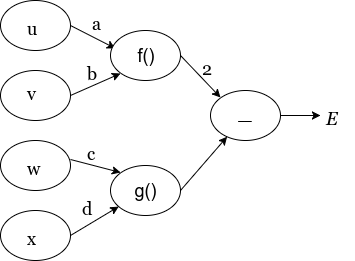
\includegraphics[scale=0.5]{download.png}
                  \end{minipage}\quad
                  \begin{minipage}{0.55\linewidth}
                  Here $u,v,w,x$ are inputs (constants) and $a,b,c,d$ are parameters (variables). $f$ and $g$ are the activation functions (with $z$ as input) defined as below:
                  \begin{eqnarray*}
                  f(z) = sigm(z) \qquad \qquad g(z) = tanh(z)
                  \end{eqnarray*}
                  \end{minipage}\\                  
                  Note that here $E$ is a function of parameters $a,b,c,d$.
                  Compute the partial derivatives of $E$ with respect to the parameters $a$, $b$, $c$ and $d$ \textit{i.e.} $\frac{\partial E}{\partial a}$, $\frac{\partial E}{\partial b}$, $\frac{\partial E}{\partial c}$ and $\frac{\partial E}{\partial d}$.
                  \begin{solution}
                  \vspace*{0mm}
                  Given, E =  2*f(au + bv) - g(cw + dx) , f(z) = sigm(z) and g(z) = tanh(z).
                  \begin{align*}
                      \therefore E &=2*sigm(au + bv)-tanh(cw + dx)\\
                      \intertext{The partial derivative of $E$ w.r.t $a$ is given by $\frac{\partial E}{\partial a}$,  which can be found as follows:}
                      \frac{\partial E}{\partial a} &= 2*\frac{\partial}{\partial a}(sigm(au+bv))\\
                      &= 2*sigm(au+bv)(1-sigm(au+bv))\frac{\partial} {\partial a}(au+bv)\hspace*{20mm}(By\,Chain\,Rule)\\
                      &= 2u*sigm(au+bv)(1-sigm(au+bv))\\
                      \intertext{The partial derivative of $E$ w.r.t $b$ is given by $\frac{\partial E}{\partial b}$,  which can be found as follows:}
                      \frac{\partial E}{\partial b} &= 2*\frac{\partial}{\partial b}(sigm(au+bv))\\
                      &= 2*sigm(au+bv)(1-sigm(au+bv))\frac{\partial} {\partial b}(au+bv)\hspace*{20mm}(By\,Chain\,Rule)\\
                      &= 2v*sigm(au+bv)(1-sigm(au+bv))\\
                      \intertext{The partial derivative of $E$ w.r.t $c$ is given by $\frac{\partial E}{\partial c}$,  which can be found as follows:}
                      \frac{\partial E}{\partial c} &= -\frac{\partial}{\partial c}(tanh(cw+dx))\\
                      &= -sech^2(cw+dx)\frac{\partial}{\partial c}(cw+dx) \hspace*{56mm}(By\,Chain\,Rule)\\
                      &= -w*sech^2(cw+dx)\\
                      \intertext{The partial derivative of $E$ w.r.t $d$ is given by $\frac{\partial E}{\partial d}$,  which can be found as follows:}
                      \frac{\partial E}{\partial d} &= -\frac{\partial}{\partial d}(tanh(cw+dx))\\
                      &= -sech^2(cw+dx)\frac{\partial}{\partial d}(cw+dx) \hspace*{56mm}(By\,Chain\,Rule)\\
                      &= -x*sech^2(cw+dx)
                  \end{align*}
                  \end{solution}
            \part Assume that $z = f(x, y)$, where $x = uv$ and $y = \frac{u}{v}$. We use $f_{x}$ to denote the partial derivative $\frac{\partial f}{\partial x}$. Using the chain rule, express  $\frac{\partial z }{\partial u}$ and  $\frac{\partial z }{\partial v}$ in terms of $u$, $v$, $f_{x}$ and $f_{y}$. 
        \begin{solution}
            \vspace*{0mm}
            Given, $z = f(x,y)$\\
            
            The partial derivative of $z$ w.r.t $u$ is given by $\frac{\partial z}{\partial u}$,  which can be found as follows:
            \begin{align*}
                \frac{\partial z }{\partial u} &= \frac{\partial f }{\partial u} = \frac{\partial f }{\partial x}\frac{\partial x }{\partial u} + \frac{\partial f }{\partial y}\frac{\partial y }{\partial u} \hspace*{40mm}(By\,Chain\,Rule)\\
                 \intertext{Substituting $\frac{\partial f }{\partial x}$ with $f_{x}$ , $\frac{\partial f }{\partial y}$ with $f_{y}$ , $x$ with $uv$ and $y$ with $\frac{u}{v}$,}
                &= f_{x} \frac{\partial}{\partial u}(uv) + f_{y} \frac{\partial}{\partial u}(\frac{u}{v})\\
                &= f_{x} v + f_{y} \frac{1}{v}\\
                \intertext{The partial derivative of $z$ w.r.t $v$ is given by $\frac{\partial z}{\partial v}$,  which can be found as follows:}
                \frac{\partial z }{\partial v} &= \frac{\partial f }{\partial v} = \frac{\partial f }{\partial x}\frac{\partial x }{\partial v} + \frac{\partial f }{\partial y}\frac{\partial y }{\partial v} \hspace*{40mm}(By\,Chain\,Rule)\\
                &= f_{x} \frac{\partial}{\partial v}(uv) + f_{y} \frac{\partial}{\partial v}(\frac{u}{v})\\
                &= f_{x} u - f_{y} \frac{u}{v^2}
            \end{align*}
        \end{solution}
            
    
    \part Given the change of variables as mentioned in the previous part: $x = uv$ and $y = \frac{u}{v}$, calculate the Jacobian of this transformation.
    \begin{solution}
    \vspace*{0mm}
        The jacobian of the transformation $x=uv$ and $y=\frac{u}{v}$ is:
        \begin{align*}
            \frac{\partial(x,y)}{\partial(u,v)} &= \begin{vmatrix} \frac{\partial x}{\partial u} & \frac{\partial x}{\partial v} \\ 
            \frac{\partial y}{\partial u} & \frac{\partial y}{\partial v}\end{vmatrix}\\
            &= \frac{\partial x}{\partial u}\frac{\partial y}{\partial v} - \frac{\partial y}{\partial u}\frac{\partial x}{\partial v}\\
            &= \frac{\partial}{\partial u}(uv)\frac{\partial}{\partial v}(\frac{u}{v}) - \frac{\partial}{\partial u}(\frac{u}{v})\frac{\partial}{\partial v}(uv)\\
            &= (v)(-\frac{u}{v^2}) -  (\frac{1}{v})(u) \\
            &= - 2*\frac{u}{v}
        \end{align*}
    \end{solution}
    \part Calculate the Jacobian of the transformation for rectangular coordinates; \textit{i.e.}, the Jacobian of $x$ = $r sin \theta$, $y$ = $r cos \theta$, $z$ = $z$, (hint: using the relevant partial derivatives)
    \begin{solution}
    \vspace*{0mm}
        The jacobian of the transformation $x=rsin\theta$, $y=rcos\theta$ and $z=z$ is:
        \begin{align*}
            \frac{\partial(x,y,z)}{\partial(r,\theta,z)} &= \begin{vmatrix}
            \frac{\partial x}{\partial r} &\frac{\partial x}{\partial \theta}  &\frac{\partial x}{\partial z} \\ 
            \frac{\partial y}{\partial r} &\frac{\partial y}{\partial \theta}  & \frac{\partial y}{\partial z}\\ 
            \frac{\partial z}{\partial r} &\frac{\partial z}{\partial \theta}  & \frac{\partial z}{\partial z} 
            \end{vmatrix}\\
            &= \begin{vmatrix}
            sin\theta & rcos\theta  & 0 \\ 
            cos\theta &-rsin\theta  & 0\\ 
            0 & 0  & 1 
            \end{vmatrix}\\
            &= -r*sin^2 \theta - r*cos^2 \theta\\
            &= -r(sin^2 \theta + cos^2 \theta)\\
            &= -r
        \end{align*}
    \end{solution}
    \end{parts}
\question  \textbf{Visit Taylor Series} The first order derivative of a function $f$ is defined by the following limit,
          \begin{equation} \label{eq:deriv_definition}
            \frac{df(x)}{dx} = \lim_{h \to 0} \frac{f(x + h) - f(x)}{h}
          \end{equation}
          On observing the above definition we see that the derivative of a function is the ratio of
          change in the function value to the change in the function input, 
          when we change the input by a small quantity (infinitesimally small).
          A first degree approximation based on eq. \ref{eq:deriv_definition} would be the following.
          \begin{equation}
            f(x+h) \approx f(x) + h \frac{df(x)}{dx}
          \end{equation}
          Consider $f(x) = ln(x+5)$. 
         \begin{parts}
         \part
          Estimate the value of $f(1)$,$f(1.1)$ and $f(2.5)$ using the above formula.
                \begin{solution}
                \vspace*{0mm}
                Given,
                    \begin{align*}
                        f(x) &= ln(x+5)\\
                        \therefore \frac{df(x)}{dx} &= f'(x) = \frac{1}{x+5}\\
                        \intertext{First degree approximation is: $f(x+h) = f(x) + h f'(x)$}
                        \intertext{Let, $x=0$ and $h=1$ then,}
                        f(1) &= f(0) + 1* f'(0)\\
                        &= ln(5) + \frac{1}{5} = 1.8094\\
                        \intertext{Let, $x=0$ and $h=1.1$ then,}
                        f(1.1) &= f(0) + 1.1* f'(0)\\
                        &= ln(5) + \frac{1.1}{5} = 1.8294\\
                        \intertext{Let, $x=0$ and $h=2.5$ then,}
                        f(2.5) &= f(0) + 2.5* f'(0)\\
                        &= ln(5) + \frac{2.5}{5} = 2.1094
                    \end{align*}
                \end{solution}
          \part Compare these estimates to the actual values of function $f(1)$,$f(1.1)$ and $f(2.5)$. Explain the discrepancy as we increase the value.
                \begin{solution}
                \vspace*{0mm}
                Actual vs estimated values of the function $f(x)=ln(x+5)$:
                \begin{center}
                    \begin{tabular}{ c c c }
                     f & Actual & Estimated \\
                     f(1) & 1.79175 & 1.8094 \\ 
                     f(1.1) & 1.80828 & 1.8294 \\  
                     f(2.5) & 2.01490  & 2.1094    
                    \end{tabular}
                \end{center}
                Here, the values are estimated by taking the derivatives at 0. It gives the tangent line to function at x = 0. So near to $x=0$ it'll give better accuracy and As we increase the value, distance between tangent line of function and actual value is increases, accuracy is decreases.\\
                \end{solution}
          \part Can we get a better estimate of $f(1)$,$f(1.1)$ and $f(2.5)$ ? How?
                \begin{solution}
                \vspace*{0mm}
                Yes, we can get better estimation of function values by taking the second order approximation as it'll add one more term, which is related to the second derivative.\\
                second order approximation is: $f(x+h) = f(x) + h f'(x)+ \frac{h^2}{2}f"(x)$.\\
                \begin{align*}
                    f(x) &= ln(x+5)\\
                    \therefore \frac{df(x)}{dx} &= f'(x) = \frac{1}{x+5}\\
                    \therefore \frac{d^2f(x)}{dx^2} &= f"(x) = -\frac{1}{(x+5)^2}\\
                        \intertext{Let, $x=0$ and $h=1$ then,}
                        f(1) &= f(0) + 1* f'(0) + \frac{1}{2}*f"(0)\\
                        &= ln(5) + \frac{1}{5} - \frac{1}{50}= 1.7894\\
                        \intertext{Let, $x=0$ and $h=1.1$ then,}
                        f(1.1) &= f(0) + 1.1* f'(0)+ \frac{(1.1)^2}{2}f"(0)\\
                        &= ln(5) + \frac{1.1}{5} - \frac{1.21}{50} = 1.8052\\
                        \intertext{Let, $x=0$ and $h=2.5$ then,}
                        f(2.5) &= f(0) + 2.5* f'(0)+ \frac{(2.5)^2}{2}f"(0)\\
                        &= ln(5) + \frac{2.5}{5} - \frac{6.25}{50} = 1.9844
                    \end{align*}
                    Second order approximation gives better estimation compared to first order approximation.
                \end{solution}
            
        \part Consider $g(x) = a + be^{x} + c*\cos(x)$. Find a, b, c $\in$ R such that $g$ approximates $f$ at
$x$ = 0. (i.e. by matching the (i) direct values (ii) first derivative and (iii) second derivative at $x = 0$).
        \begin{solution}
        \vspace*{0mm}
        \begin{align*}
            g(x) &= a + be^{x} + c*\cos(x)\\
            \therefore \frac{dg(x)}{dx} &= g'(x) = be^{x} - c*\sin(x)\\
            \therefore \frac{d^2g(x)}{dx^2} &= g"(x) = be^{x} - c*\cos(x)\\
            \intertext{And,}
            f(x) &= ln(x+5)\\
            \therefore \frac{df(x)}{dx} &= f'(x) = \frac{1}{x+5}\\
            \therefore \frac{d^2f(x)}{dx^2} &= f"(x) = -\frac{1}{(x+5)^2}\\
            \intertext{By comparing direct value of functions at $x=0$,}
            g(0)&=f(0)\\
            a+b+c &= ln(5) \hspace*{50mm}(1)\\
            \intertext{By comparing first derivative of functions at $x=0$,}
            g'(0)&=f'(0)\\
            b &= \frac{1}{5} = 0.2\\
            \intertext{By comparing second derivative of functions at $x=0$,}
            g"(0)&=f"(0)\\
            b-c &= -\frac{1}{25}\\
            \therefore c &= b + \frac{1}{25}\\
            \therefore c &= \frac{6}{25} = 0.24\\
            \intertext{Now, putting values of b and c into equation(1),}
            a &= ln(5) - 0.2 -0.24 \\
            \therefore a &= 1.16944
        \end{align*}
        \end{solution}
          
\end{parts}

\question
\textbf{Differentiation of function of multiple variables}
          \begin{equation*}
            \begin{aligned}
              s_1 & = tan(w_1 x) \\
              s_2 & = sec(w_2 x + s_1) \\
              s_3 & = sin(w_3 s_1 + w_4 s_2) \\
              s_4 & = cos(w_5 s_3 + w_6) \\
              y   & = tanh(w_7 s_4 + w_8)
            \end{aligned}
          \end{equation*}

          An alternative representation of the function $y$ is given in the figure below.
          \begin{center}
            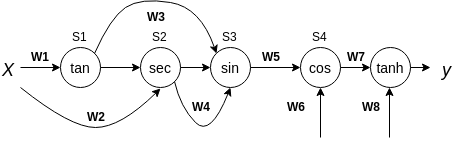
\includegraphics[scale=0.7]{fig2.png}
          \end{center}

          Compute the derivatives $\frac{dy}{dw_1}$ and $\frac{dy}{dw_2}$ (show all the steps).

          \begin{solution}
          \vspace*{0mm}
          The derivative of $y$ w.r.t $w_1$ is given by $\frac{dy}{dw_1}$,  which can be found as follows:
          \begin{align*}
            \frac{dy}{dw_1} &= \frac{d}{dw_1}(tanh(w_7 s_4 + w_8))\\
            &= sech^2(w_7 s_4 + w_8)\frac{d}{dw_1}(w_7 s_4 + w_8)\\
            &= sech^2(w_7 s_4 + w_8)(w_7\frac{d}{dw_1}(cos(w_5 s_3 + w_6)))\\
            &= -w_7 sech^2(w_7 s_4 + w_8)sin(w_5 s_3 + w_6) \frac{d}{dw_1}(w_5 s_3 + w_6)\\
            &= -w_7 sech^2(w_7 s_4 + w_8)sin(w_5 s_3 + w_6) (w_5 \frac{d}{dw_1}sin(w_3 s_1 + w_4 s_2))\\
            &= -w_5 w_7 sech^2(w_7 s_4 + w_8)sin(w_5 s_3 + w_6) cos(w_3 s_1 + w_4 s_2)\frac{d}{dw_1}(w_3 s_1 + w_4 s_2)\\
            &= -w_5 w_7 sech^2(w_7 s_4 + w_8)sin(w_5 s_3 + w_6) cos(w_3 s_1 + w_4 s_2)\\
            & \qquad(w_3 \frac{d}{dw_1}tan(w_1 x) + w_4 \frac{d}{dw_1}sec(w_2 x + s_1))\\
            &= -w_5 w_7 sech^2(w_7 s_4 + w_8)sin(w_5 s_3 + w_6) cos(w_3 s_1 + w_4 s_2)\\
            & \qquad(w_3 sec^2(w_1 x)\frac{d}{dw_1}(w_1 x) + w_4 sec(w_2 x + s_1)tan(w_2 x + s_1)\frac{d}{dw_1}(w_2 x + s_1))\\
            &= -w_5 w_7 sech^2(w_7 s_4 + w_8)sin(w_5 s_3 + w_6) cos(w_3 s_1 + w_4 s_2)\\
            & \qquad(w_3 x sec^2(w_1 x) + w_4 sec(w_2 x + s_1)tan(w_2 x + s_1)\frac{d}{dw_1}(tan(w_1 x)))\\
            &= -w_5 w_7 sech^2(w_7 s_4 + w_8)sin(w_5 s_3 + w_6) cos(w_3 s_1 + w_4 s_2)\\
            & \qquad(w_3 x sec^2(w_1 x) + w_4 x sec(w_2 x + s_1)tan(w_2 x + s_1)sec^2(w_1 x))\\
            &= -x w_5 w_7 sech^2(w_7 s_4 + w_8)sin(w_5 s_3 + w_6) cos(w_3 s_1 + w_4 s_2) sec^2(w_1 x)\\
            & \qquad(w_3 + w_4 sec(w_2 x + s_1)tan(w_2 x + s_1))\\
            \intertext{The derivative of $y$ w.r.t $w_2$ is given by $\frac{dy}{dw_2}$,  which can be found as follows:}
            \frac{dy}{dw_2} &= \frac{d}{dw_2}(tanh(w_7 s_4 + w_8))\\
            &= sech^2(w_7 s_4 + w_8)\frac{d}{dw_2}(w_7 s_4 + w_8)\\
            &= sech^2(w_7 s_4 + w_8)(w_7\frac{d}{dw_2}(cos(w_5 s_3 + w_6)))\\
            &= -w_7 sech^2(w_7 s_4 + w_8)sin(w_5 s_3 + w_6) \frac{d}{dw_2}(w_5 s_3 + w_6)\\
            &= -w_7 sech^2(w_7 s_4 + w_8)sin(w_5 s_3 + w_6) (w_5 \frac{d}{dw_2}sin(w_3 s_1 + w_4 s_2))\\
            &= -w_5 w_7 sech^2(w_7 s_4 + w_8)sin(w_5 s_3 + w_6) cos(w_3 s_1 + w_4 s_2)\frac{d}{dw_2}(w_3 s_1 + w_4 s_2)\\
            &= -w_5 w_7 sech^2(w_7 s_4 + w_8)sin(w_5 s_3 + w_6) cos(w_3 s_1 + w_4 s_2)\\
            & \qquad(w_3 \frac{d}{dw_2}tan(w_1 x) + w_4 \frac{d}{dw_2}sec(w_2 x + s_1))\\
            &= -w_5 w_7 sech^2(w_7 s_4 + w_8)sin(w_5 s_3 + w_6) cos(w_3 s_1 + w_4 s_2)\\
            & \qquad( w_4 sec(w_2 x + s_1)tan(w_2 x + s_1)\frac{d}{dw_2}(w_2 x + s_1))\\
            &= -x w_4 w_5 w_7 sech^2(w_7 s_4 + w_8)sin(w_5 s_3 + w_6) cos(w_3 s_1 + w_4 s_2)\\
            & \qquad sec(w_2 x + s_1)tan(w_2 x + s_1)
          \end{align*}
          \end{solution}
          
\question \textbf{Differentiation of vectors/matrices}
          \newline
          Consider vectors $\boldsymbol{u,b} \in \mathbb{R}^d$, and matrix $\boldsymbol{A} \in \mathbb{R}^{n \times n}$.
          \newline
          The derivative of a scalar $f$ w.r.t. a vector $\boldsymbol{u}$ is a vector by itself, given by
          \[
            \nabla f = \left( \frac{\partial f}{\partial u_1}, \frac{\partial f}{\partial u_2}, \dots, 
                         \frac{\partial f}{\partial u_n} 
                       \right)
          \]
          \newline
         ( \textbf{Hint}:  The derivative of a scalar $f$ w.r.t. a matrix $\boldsymbol{X}$, is a matrix whose $(i,j)$ component is $\frac{\partial f}{\partial X_{ij}}$, where $X_{ij}$ is the $(i,j)$ component of the matrix $\boldsymbol{X}$.)
         \newline
         \begin{parts}
         \part Derive the expression for the derivative:  $ \nabla \textbf{\textit{u}}^{T}\textbf{\textit{Au}} + \textbf{\textit{b}}^{T}\textbf{\textit{u}}$.
         \begin{solution}
         \vspace*{0mm}
         The derivation of above equation can be given as follows:
         \begin{align*}
            \nabla {u}^{T}{Au} + {b}^{T}{u} &= \frac{\partial}{\partial u}({u}^{T}{Au}) + \frac{\partial}{\partial u}({b}^{T}{u})\\
            &= {u}^{T}({A}^{T}+{A}) + {b}^{T}\\
            \intertext{if matrix A is symmetric then we can write above equation as:}
            &= 2{u}^{T}{A} + {b}^{T}
         \end{align*}
         \end{solution}
         \part Compare your results with derivatives for the scalar equivalents
          of the above expressions $au^{2}+ bu$.
         \begin{solution}
         \vspace*{0mm}
         The derivation of scalar equation $au^{2}+ bu$ can be given as follows:
         \begin{align*}
             \frac{\partial}{\partial u}(au^{2}+ bu) &=\frac{\partial}{\partial u}(au^{2})+ \frac{\partial}{\partial u}(bu)\\
             &= 2au+b 
         \end{align*}
         The above obtained result is similar to the result of expression in part(a) if matrix A is symmetric.
         \end{solution}
         \part Derive the Hessian: $\frac{\partial^{2}f}{\partial \textbf{u}\partial \textbf{u}^{T}}$ given that $f = \textbf{\textit{u}}^{T}\textbf{\textit{Au}} + \textbf{\textit{b}}^{T}\textbf{\textit{u}}$
         \begin{solution}
         \vspace*{0mm}
         The Hessian of the given expression can be found as follows:
         \begin{align*}
             \nabla^2 {u}^{T}{Au} + {b}^{T}{u} &= \frac{\partial}{\partial u}( \frac{\partial}{\partial u}({u}^{T}{Au} + {b}^{T}{u})) \\
             &=\frac{\partial}{\partial u}( \frac{\partial}{\partial u}({u}^{T}{Au}) + \frac{\partial}{\partial u}({b}^{T}{u}))\\
            &= \frac{\partial}{\partial u}({u}^{T}({A}^{T}+{A}) + {b}^{T})\\
            &= {A}^{T}+{A}
         \end{align*}
         \end{solution}
         
         \end{parts}
\question \textbf{Encoding Tongue Twister :} You have been assigned a task to encode a tongue-twister
phrase compactly:
`clean clams crammed in clean clans'.
For convenience, you are given the frequency distribution as below.
\begin{table*}[h]
    \centering
    \begin{tabular}{c|c}
        \toprule
         Char & Frequency  \\
         \midrule
         a & 5\\
         c & 5 \\
         d & 1 \\
         e & 3 \\
         i & 1 \\
         l & 4 \\
         m & 3 \\
         n & 4 \\
         r & 1 \\
         s & 2 \\
         space & 5\\
         \bottomrule
    \end{tabular}
    \label{tab1}
\end{table*}
\begin{parts}
\part One way to encode this sequence is to use fixed length code with each code word long enough to encode ten different symbols. How many
bits
would
be
needed
for
this
34-character
phrase
using
such
a
fixed-length
code?
\begin{solution}
\vspace*{0mm}
Encode using fixed length code:\\
There are ten different symbols so we'll need 4 bits to represent each character.
\begin{align*}
    \therefore total\,number\,of\,bits\,needed\,for\,34-character\, is &= 34*4\,bits\\
    &= 136 \,bits
\end{align*}
\end{solution}
\part What are the
minimum
number
of
bits
needed (theoretically)
to
encode
the
entire
phrase
,
assuming
that
each
character
is
independent
of
the
surrounding
character? 
Hint: We can calculate the average information (in other words, bits needed) of a symbol using entropy information.
\begin{solution}
\vspace*{0mm}
Encode using entropy information:\\
The Shannon entropy H gives number of bits needed per symbol and is given by:$H = -\sum_{k}{} p_{k}\log_{2}p_{k}$\\
where, $p_{k}$ is the probability of occurrence of the k-th possible symbol.\\
Here, we have ten different symbols.
\begin{align*}
\therefore\,&Average\,number\,of\,bits\,needed\,for\,a\,character\,is:\\     
    H &= -\sum_{k=1}^{10} p_{k}\log_{2}p_{k}\\
    &= -(\frac{5}{34}\log_{2}(\frac{5}{34}) + \frac{5}{34}\log_{2}(\frac{5}{34})+ \frac{1}{34}\log_{2}(\frac{1}{34})+ \frac{3}{34}\log_{2}(\frac{3}{34})+ \frac{1}{34}\log_{2}(\frac{1}{34}) \\
    &\qquad +\frac{4}{34}\log_{2}(\frac{4}{34})+ \frac{3}{34}\log_{2}(\frac{3}{34}) + \frac{4}{34}\log_{2}(\frac{4}{34})+ \frac{1}{34}\log_{2}(\frac{1}{34}) + \frac{2}{34}\log_{2}(\frac{2}{34})\\
    &\qquad + \frac{5}{34}\log_{2}(\frac{5}{34}))\\
    &= -(\frac{15}{34}\log_{2}(\frac{5}{34}) +  \frac{3}{34}\log_{2}(\frac{1}{34})+ \frac{6}{34}\log_{2}(\frac{3}{34})+ \frac{8}{34}\log_{2}(\frac{4}{34})+ \frac{2}{34}\log_{2}(\frac{2}{34}))\\
    &= 3.25397\\
    \therefore\,&minimum\,number\,of\,bits\,needed\,to\,encode\, 33-characters\,is=\ceil*{34*(3.25397)}\\
    &= \ceil*{110.63498}\\
    &= 111\,bits\\
    \intertext{So, minimum number of bits needed to encode  33-characters is 111 bits.}
\end{align*}
\end{solution}
\end{parts}
\question \textbf{Plotting Functions for Great Good}
          \begin{parts}
            \part Consider the variable $x$ and functions $h_{11}(x)$, $h_{12}(x)$ and $h_{21}(x)$ such that

                  \begin{align*}
                    h_{11}(x) = \frac{1}{1 + e^{-(500 x + 30)}}  \\
                    h_{12}(x) = \frac{1}{1 + e^{-(500 x - 30)}}  \\
                    h_{21} = h_{11}(x) - h_{12}(x)  \\
                  \end{align*}
                  The above set of functions are summarized in the graph below.
                  \begin{center}
            		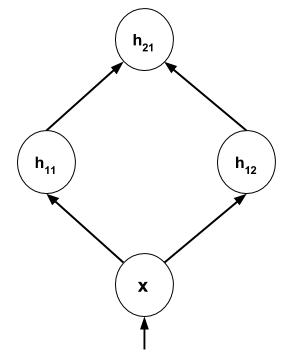
\includegraphics[scale=0.35]{sig2d}
          		  \end{center}
                  Plot the following functions: $h_{11}(x)$, $h_{12}(x)$ and $h_{21}(x)$ for $x \in (-1, 1)$
            \begin{solution}
            \vspace*{0mm}
            Plot of the functions:\\ 
                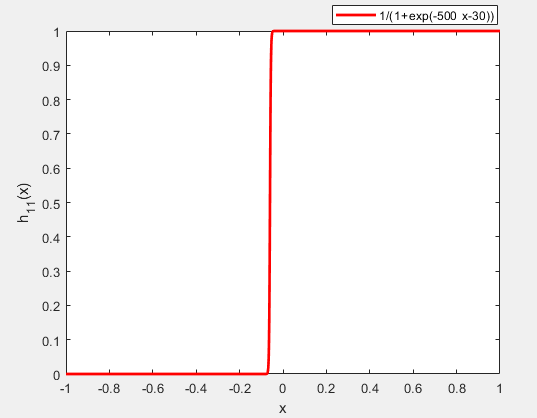
\includegraphics[width=7cm,height=5cm]{1}
                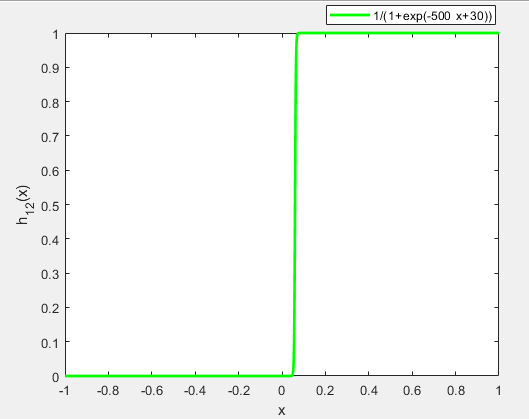
\includegraphics[width=7cm,height=5cm]{2}\\
                \hspace*{30mm}$h_{11}(x)$ \hspace*{60mm} $h_{12}(x)$\\
                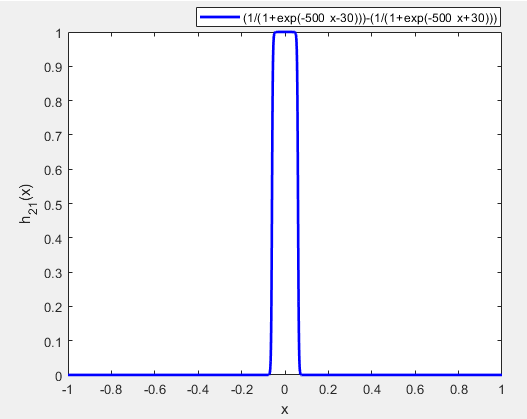
\includegraphics[width=7cm,height=5cm]{3}\\
                \hspace*{30mm}$h_{21}(x)$
            \end{solution}

            \part Now consider the variables $x_1, x_2$ and the functions $h_{11}(x_1, x_2), h_{12}(x_1, x_2), h_{13}(x_1, x_2), h_{14}(x_1, x_2)$, $h_{21}(x_1, x_2), h_{22}(x_1, x_2), h_{31}(x_1, x_2)$ and $f(x_1, x_2)$ such that   
   
                  \begin{align*}
                    h_{11}(x_1, x_2) &= \frac{1}{1 + e^{-(x_1 + 50x_2 + 100)}}  \\
                    h_{12}(x_1, x_2) &= \frac{1}{1 + e^{-(x_1 + 50x_2 - 100)}}  \\
                    h_{13}(x_1, x_2) &= \frac{1}{1 + e^{-(50x_1 + x_2 + 100)}}  \\
                    h_{14}(x_1, x_2) &= \frac{1}{1 + e^{-(50x_1 + x_2 - 100)}}  \\
                    h_{21}(x_1, x_2) &= h_{11}(x_1, x_2) - h_{12}(x_1, x_2)\\
                    h_{22}(x_1, x_2) &= h_{13}(x_1, x_2) - h_{14}(x_1, x_2)\\
                    h_{31}(x_1, x_2) &= h_{21}(x_1, x_2) + h_{22}(x_1, x_2)\\
                    f(x_1, x_2) &= \frac{1}{1 + e^{-(100h_{31}(x) - 200)}}  \\\\
                  \end{align*}
                  The above set of functions are summarized in the graph below.
                    \begin{center}
            		  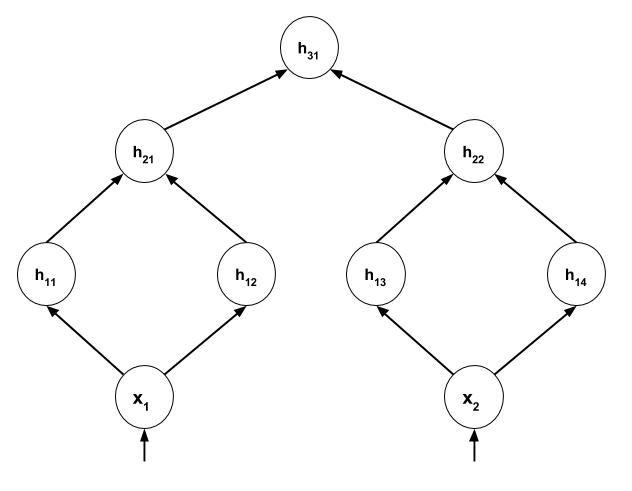
\includegraphics[scale=0.35]{sig3d}
          		    \end{center} 
                  Plot the following functions: $h_{11}(x_1, x_2), h_{12}(x_1, x_2), h_{13}(x_1, x_2), h_{14}(x_1, x_2), h_{21}(x_1, x_2),$ $h_{22}(x_1, x_2), h_{31}(x_1, x_2)$ and $f(x_1, x_2)$ for $x_1 \in (-5, 5)$ and $x_2 \in (-5, 5)$
            \begin{solution}
            \vspace*{0mm}
            Plot of the functions:\\ 
            
                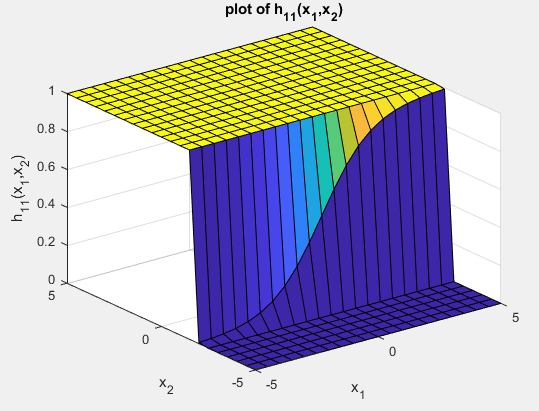
\includegraphics[width=7cm,height=5cm]{4}
                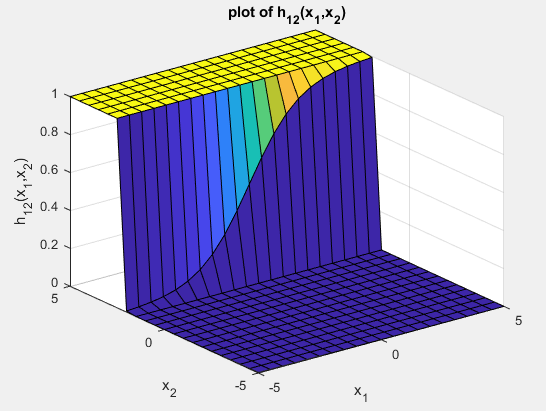
\includegraphics[width=7cm,height=5cm]{5}\\

                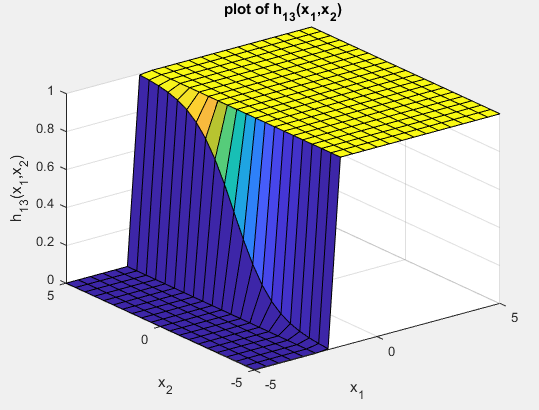
\includegraphics[width=7cm,height=5cm]{6}
                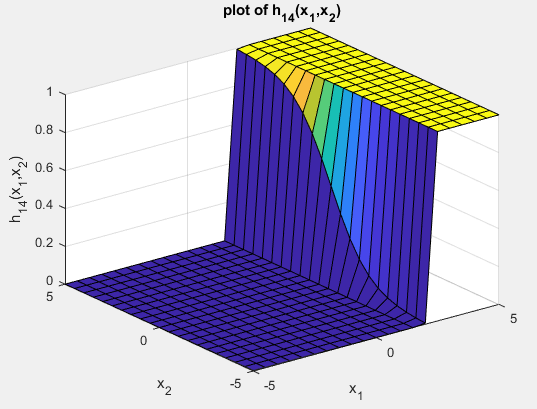
\includegraphics[width=7cm,height=5cm]{7}\\
                
                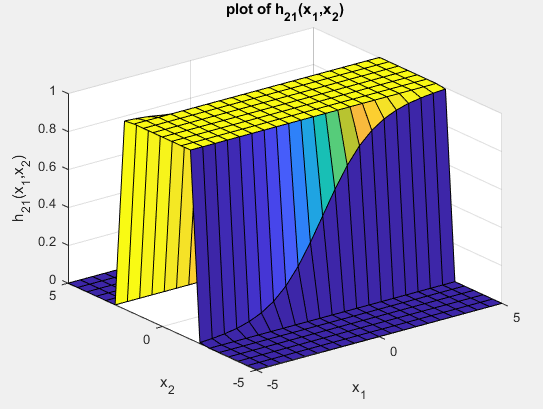
\includegraphics[width=7cm,height=5cm]{8}
                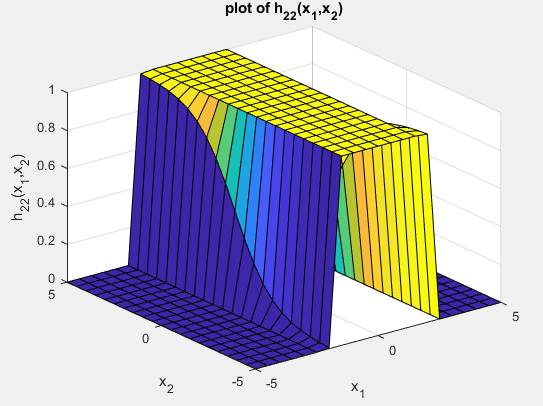
\includegraphics[width=7cm,height=5cm]{9}\\
                
                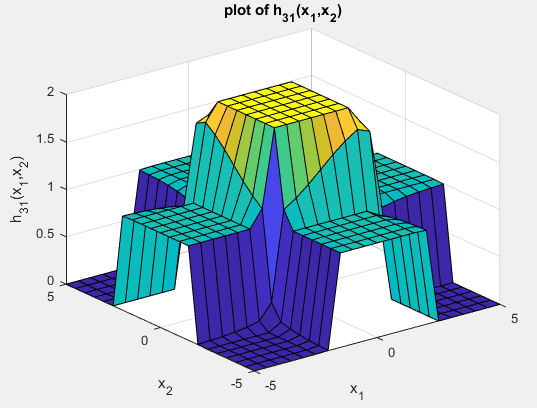
\includegraphics[width=7cm,height=5cm]{10}
                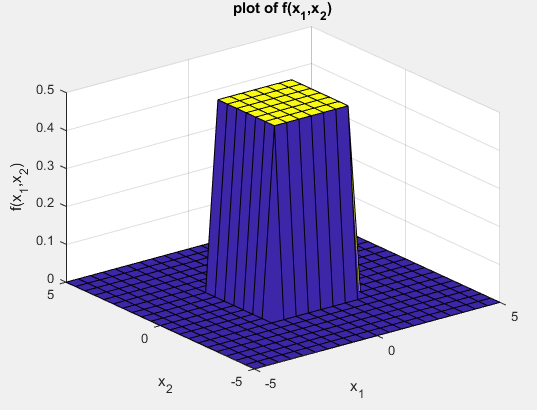
\includegraphics[width=7cm,height=5cm]{11}\\
                
            \end{solution}
                 
           \end{parts}
\end{questions}             
\end{document}
